\section{Introduction}

Ever-increasing capabilities of data collection techniques (i.e. genetic sequencing, geographic information systems monitoring, and etc) and sampling efforts from field biologist are making large volumes of ecological/biological data available over an ever-wider range of species and also higher resolution (i.e. measurable phenotypic traits to genetic sequence data). 
As a result, researchers are interested in exploring ways to study more complicated systems and fitting more models to data or synthetic databases of species traits.
One particular area of interest in ecological/evolutionary statistics is phylogenetic comparative analysis using phylogenetic (eco-evolutionary) regression; that is, analyzing evolutionary relationships (signals) among species between species traits and environmental variables when estimating the effects of traits within a community.
Although there are sophisticated statistical tools specially designed for this type of problem, the current state of the art of these tools are either inflexible, or computationally inefficient and unpractical when fitting large volumes of data.
In particular, modelling and understanding relationships between response and multiple predictor variables, and accounting for different levels of variation (errors) to complicated systems with large data is always challenging both biologically and statistically, and adding phylogenetic relationships will further increases the difficulties. 
In such case, researchers often try to find ways to simplify or revert to simpler models (i.e. model reduction or ignore phylogenetic relationships, or both) for practical uses \cite{bunnefeld2012island, ord2010adaptation}, which can lead to both statistical and biological issues \cite{felsenstein1985phylogenies, li2017statistical}. 
In this paper, we propose an alternative method that can flexibly and computational efficiently model phylogenetic relationships via mixed effect models, highlighting various complexities of phylogenetic relationships through random effects.
We will use this modelling framework to present and discuss importance of different levels of variations and their considerations and interpretations in phylogenetic comparative analysis.

There are two general challenges in linking the evolutionary process to a phylogenetic comparative statistical framework.
First, a method for linking phylogenetic relationships among species when estimating the effects of traits. 
The standard/classic phylogenetic regression is a correlated-residual model using phylogenetically independent contrasts (PICs), where the residuals evolve as a Brownian motion process \citep{felsenstein1985phylogenies}; in other words, the variation of residuals are phylogenetically correlated.
Many of the more recent approaches -- including phylogenetic generalized linear mixed models (PGLMM) \citep{ives2011generalized}, Pagel's $\lambda$ \citep{pagel1999inferring}, and Blomberg's $K$ \citep{blomberg2003testing} -- are built upon Felsentein's PICs model by making additional sophisticated assumptions allowing extra parameters to correct for possible bias where they separate/partition the phylogenetically correlated residual variation into phylogenetically uncorrelated residual variation (observation error or tip variation) and phylogenetic signal (biological/evolutionary process error) \cite{hansen2012interpreting}.
However, when multiple observations (or repeated measures) of the same species (taxon) are being observed, this introduces another level of variation; in this case, phylogenetic signal and tip variation are now both part of the evolutionary process error and residual variation is associated with observation level variation (the standard statistical definition). 
Despite the addition of multiple observations being straightforward statistically, it is rarely seen in the literature as existing platforms are unable to fit multiple observations, or unbalanced design data, or both.

The second challenge is flexibly-incorporating modelling phylogenetic relationships to other common statistical features with many predictor variables in phylogenetic regression (i.e. phylogenetically correlated slopes, interactions, nested designs and etc.)
For example, \cite{nowakowski2018phylogenetic} considered phylogenetically correlated slopes in response to habitat conversion when studying the abundance of amphibian species, \cite{li2017canfun} considered phylogenetically correlated species nested within sites for plant abundance. 
The tools available for extending phylogenetic relationships to common statistical regression features are very limited, inflexible and computationally inefficient; thus, sophisticated biologist would turn to more flexible settings (e.g. Bayesian models).

In this paper, we will propose an alternative formulation of phylogenetic generalized linear mixed models that is mathematically equivalent to previous approaches. 
More specifically, we will show our new formulation is more flexible and can be easily extended along with the features of mixed model such as multiple observational designs, phylogenetically phylogenetic relationship on other predictor variables with random slopes (i.e. phylogenetic signal in response to change in the predictor variable), random interactions \ml{why not? we are already using this for the alternative formulation of nested RE} and nested random effect models.
We will compare our technique with existing methods to show robustness and efficiency via simulations and data.
We will end off by discussing opportunities and practicalities of our method and reevaluate the state of art for this area of research. 

\section{Materials and Methods}

The typical phylogenetic regression is of the form:
\begin{align}
y & = XB + \epsilon \label{eq:gls1} \\ 
\epsilon & \sim \textrm{MVN}(0,\sigma^{2}C), \label{eq:gls2}
\end{align}
where $y$ is an $n \times 1$ vector of measurable response; $X$ is an $n \times m$ model matrix containing 1's in the first column and the $m$ predictor variables (phenotypic traits or environmental variables); $B$ is an $m$ vector of coefficients; $\epsilon$ is the residual error and assumed to be multivariate normally distributed with a variance-covariance matrix given by $\sigma^{2}_{\epsilon}C$ in which $C$ is an $n \times n$ matrix of the phylogenetic correlation (PC).
The PC matrix is inferred from the topology of the evolutionary tree by capturing the evolutionary changes that occurred on all the branches, which can be incorporated in statistical methods.

% More recently, researchers use linear mixed model and generalized linear mixed model framework to model complex systems with phylogenetic structures.
%\ml{Why? Data type, interactions, random effects, etc... Need to really explain random effects here. Alternatively, we can drop this line and write this...}
An alternative modelling approach is to use linear mixed effects modelling framework \citep{lynch1991methods}.
The typical linear mixed model has the form:
\begin{align}
Y & \sim F(\mu) \label{eq:glmm1} \\
g(\mu) & = XB + Zb + \epsilon_{mm} \label{eq:glmm2} \\
\epsilon_{mm} & \sim \textrm{MVN}(0,\sigma^2) \label{eq:glmm3}
\end{align}
where $Z$ is an $n \times m$ model matrix for the $m$ -- dimensional vector-valued $m$ predictor variables; $\epsilon_{mm}$ is the residual error and assumed to be multivariate normally distributed with a variance-covariance matrix given by $\sigma_{2}I$.
Analogously, the phylogenetic regression given by (1) can be represented in the mixed model framework by constraining $\epsilon_{mm} = 0$, $Z$ to an $n \times 1$ matrix such that: 

\begin{align}
Z & \sim \textrm{MVN}(0,\sigma^{2}C). \label{eq:glmmgls}
\end{align}

\subsection{Reformulating phylogenetic correlation matrix}
% The standard problem of phylogenetic comparative methods is to analyze relationships among data where the observations are gathered from nodes (usually tips) of a phylogenetic tree.
% Phylogenetic independent contrasts is a generalization of the paired comparisons method where contrasts are taken for each bifurcation (nodes) in a phylogenetic tree. 
% Assuming that traits evolve independently in each lineage following speciation, then the trait divergences that occur at one node are independent of divergence at other nodes.  

An alternative approach is to model the phylogenetic correlation as a \textit{Gaussian process}. 
In particular, suppose that the evolutionary process is a Brownian motion, which means the evolution of a continuous trait is a random walk and daughter species after speciation are all independent.  
In that case, the phylogenetic variability of a particular observation can be written as the sum of the evolutionary changes that occurred on all of the branches in the phylogeny in its past. 
Thus, the evolutionary history for each species can be modeled with a sequence of independent errors with species--branch matrix $S$, rather than having to impose a correlation $C$. 
This is mathematically equivalent under BM assumption where we can reconstruct C by matrix multiplying $S$ by itself.

The random-effect model matrix $Z$ can be decomposed into term-wise model matrix $Z_{i}$ as described in \citet{bates2015fitting}.
Thus, the phylogenetic correlated random-effect matrix $Z^{C}_{i}$ is

\begin{equation}
Z^{C}_{i} = (S^{T}_{i}J^{T}_{i} \ast X^{T}_{i})^{T}, \label{eq:ZC}
\end{equation}


where $\ast$ is the Khatri-Rao product, $S_{i}$ is an $l_{i} \times b_{i}$ matrix of species--branch relations; $J_{i}$ the indicator matrix of grouping factors indices matrix size $n \times l_{i}$; $X_{i}$ is the raw random effects model matrix size $n \times p_{i}$. 

\subsection{Simulation}

We generated test data based on the simple mixed model formulation \ref{eq:glmm1}, \ref{eq:glmm2}, \ref{eq:glmm3} with a single response variable $Y$ and a single predictor continuous variable $X$ for $n$ (20, 100, and 500) species, and $m$ (1 and 20) sites/groups. 
To account for multiple levels of phylogenetic signals, we assume phylogenetic signals in the intercept $b_0$, and slope $b_1$.
We further assume that random slope and intercept are correlated. 
For models with multiple sites, we also assume for species and site interactions random effects, an equivalent version of nested random effects or phylogenetic attraction described in \cite{helmus2007separating} with the main random effects.

\subsection{Platforms}

Our algorithmic approach is general and could be implemented in a wide range of computational platforms that support independent latent variables, we implemented our approach using the lme4 R package \citep{bates2015fitting}.
We have included three additional R packages that can fit phylogenetic comparative models under BM process assumption, and they are nlme \citep{pinheiro2014r}, phylolm \citep{ho2014phylolm}, and pez \citep{pearse2015pez}.
Phylogenetic generalized least squares (PGLS) in \textit{nlme}, is one of the most widely used techniques in phylogenetic comparative analysis; it allows for the analysis of relationships among species traits in its residual variance and can also handle multiple predictor variables.
Phylogenetic generalized linear model (PGLM) in \textit{phylolm}, is a slightly more flexible variation of PGLS that can allow for within species variation (sometimes called the tip variation). 
Neither PGLS nor PGLM can fit random slope or multiple sites. 
One of the relatively few packages that currently fit random slopes or multiple sites is \textit{pez}, which can handle adding additional uncorrelated random slopes with intercept and species in multiple sites/groups.  


% Table \ml{ref something} provides the statistically equivalent fitting capabilities of common/existing phylogenetic methods.

% % \begin{table}
% % \begin{center}
% 
% \begin{tabularx}{\textwidth}{|X|X|X|}
% \hline
% Type of RE	& Formula	& Platform	\\
% \hline
% 
% Single site intercept	  &	1 $\mid$ sp	& gls (if residual = 0), phyloglm, lme4 \\
% Single site intercept and uncorrelated slopes		&  1 $\mid$ sp + trait $\mid$ sp		& lme4 \\
% Single site intercept and correlated slopes 			& 1 + trait $\mid$ sp					& lme4 \\
% \hline
% Multiple site intercept 									&  1 $\mid$ sp 						& pez, lme4 \\
% Multiple site intercept and uncorrelated slopes 	&  1 $\mid$ sp + trait $\mid$ sp 		& pez, lme4 \\
% Multiple site intercept and correlated slopes 	& 	1 + trait $\mid$ sp					& lme4 \\
% \hline
% \end{tabularx}
% % \vspace{1in}
% % ditto with site interaction								& ditto above $\mid$ sp:site		& ditto above \\
% % \end{center}
% % \end{table}

\section{Results}

\begin{center}
\begin{figure}[h]
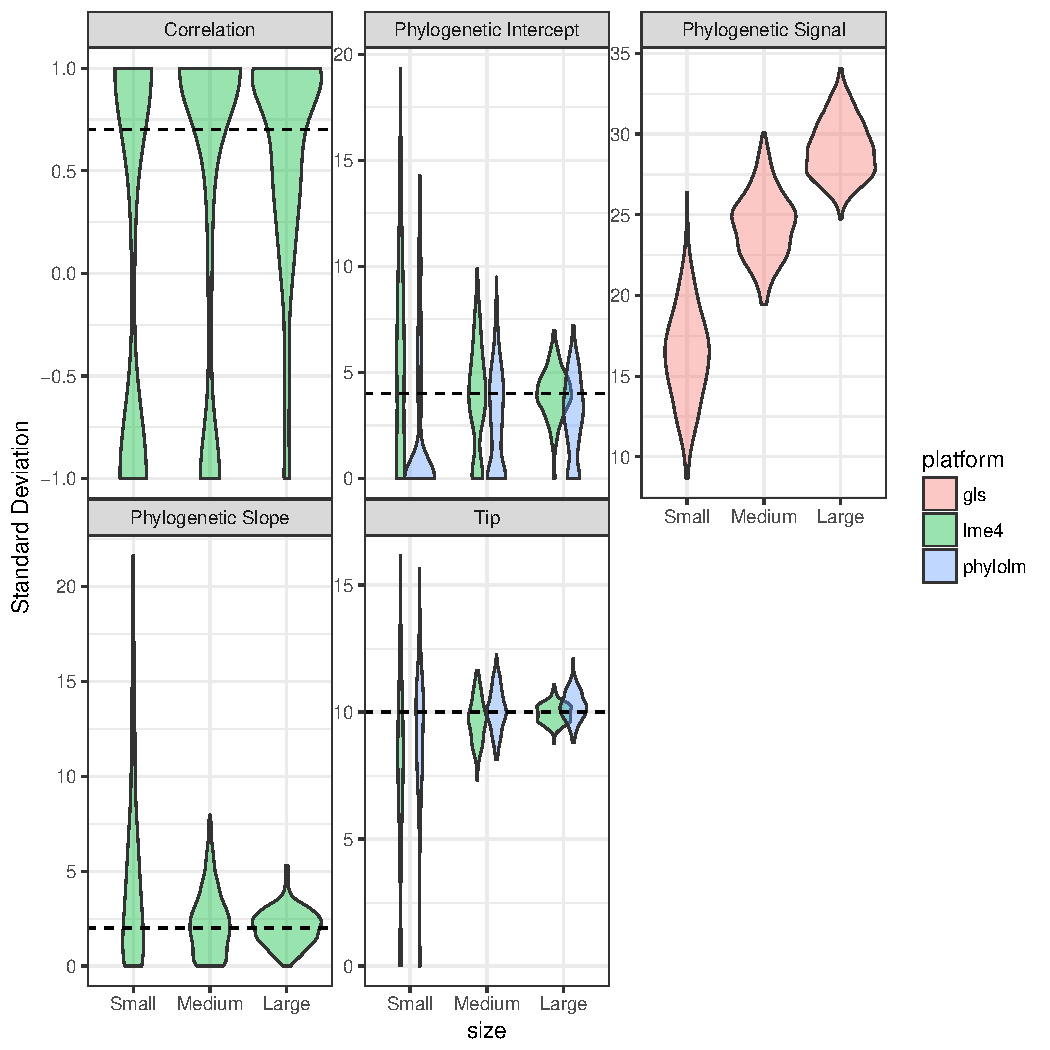
\includegraphics[scale=0.8,page=1]{./git_push/ssplot.pdf}
\label{ssplot}
\end{figure}
\end{center}

The full model (which matches the simulation model that incorporates phylogenetic signal on the intercept, slope and correlation) provides good estimates of the different levels of the phylogenetic variation signal (Figure 1 and 2).

In general, all phylogenetic signal estimates are more robust for all models (including models without random slope and correlation) with more data, except PGLS in the single site simulations. 
It is unclear how different levels of phylogenetic signal are being confounded under the error free (without tip variation) assumption for the PGLS models.
Models with only two parameters/levels of variation capture the phylogenetic intercept and tip variation reasonably well to the simulated parameters despite not including phylogenetic random slope and slope intercept correlation.

Platforms using the mixed model framework for multiple site simulations follows similar behaviour as single site simulation (i.e. different levels of phylogenetic signals and variations are closer to the simulated parameters with more data). 
All parameter estimates are much more robust for the multiple site than the single site simulations, especially slope-intercept correlations. 
There are no clear difference with phylogenetic signal models without random slope and intercept correlation.
However, despite the similarities of robustness estimation, the efficiency (measured by computational speed) of sampling independent errors in lme4 is dramatically better (orders of magnitude faster than pez.
Furthermore, it was not practical for pez to fit large sample size simulation data as the computational speed did not scale linearly.

\begin{center}
\begin{figure}[h]
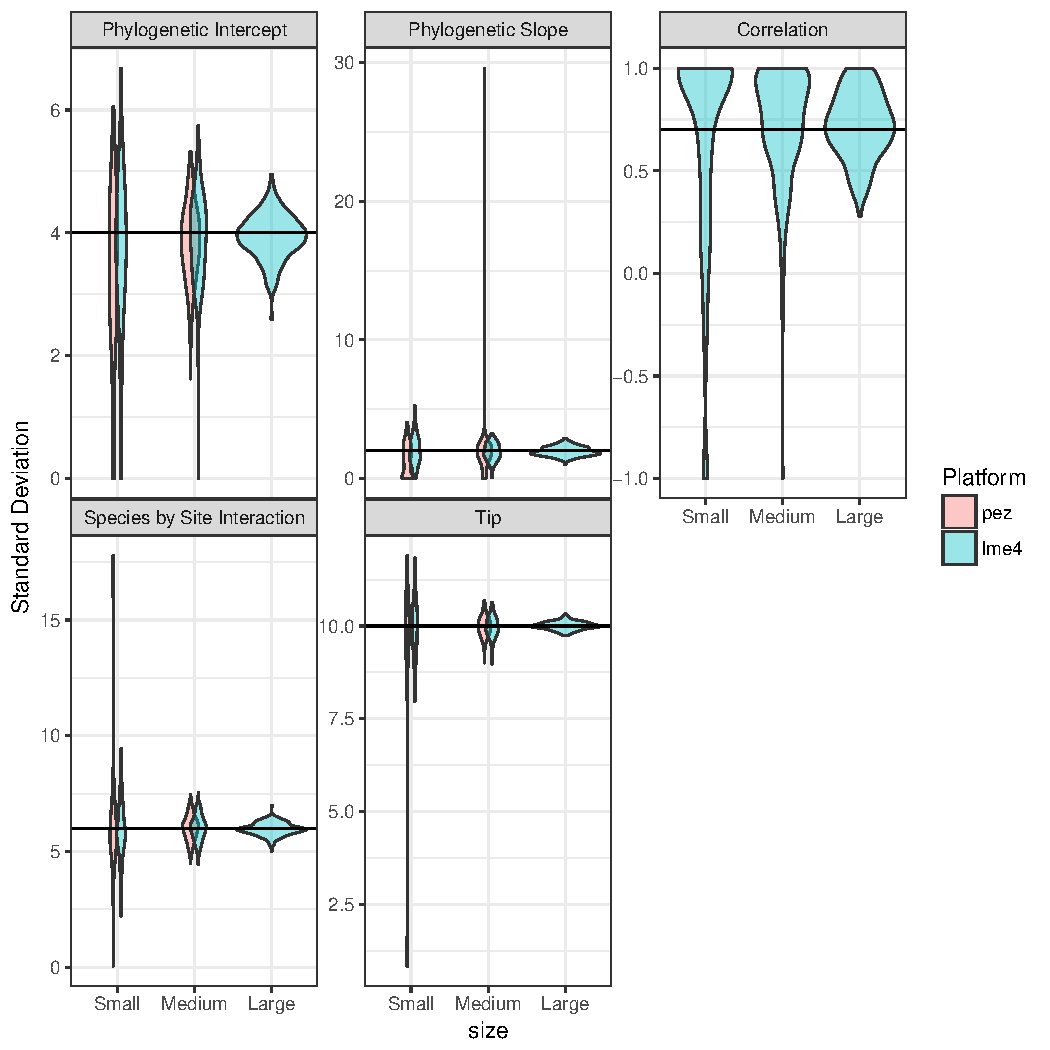
\includegraphics[scale=0.8,page=1]{./csplot.pdf}
\end{figure}
\end{center}

\begin{center}
\begin{figure}[h]
\includegraphics[scale=0.8,page=2]{./csplot.pdf}
\end{figure}
\end{center}

% \begin{center}
% \begin{figure}[h]
% 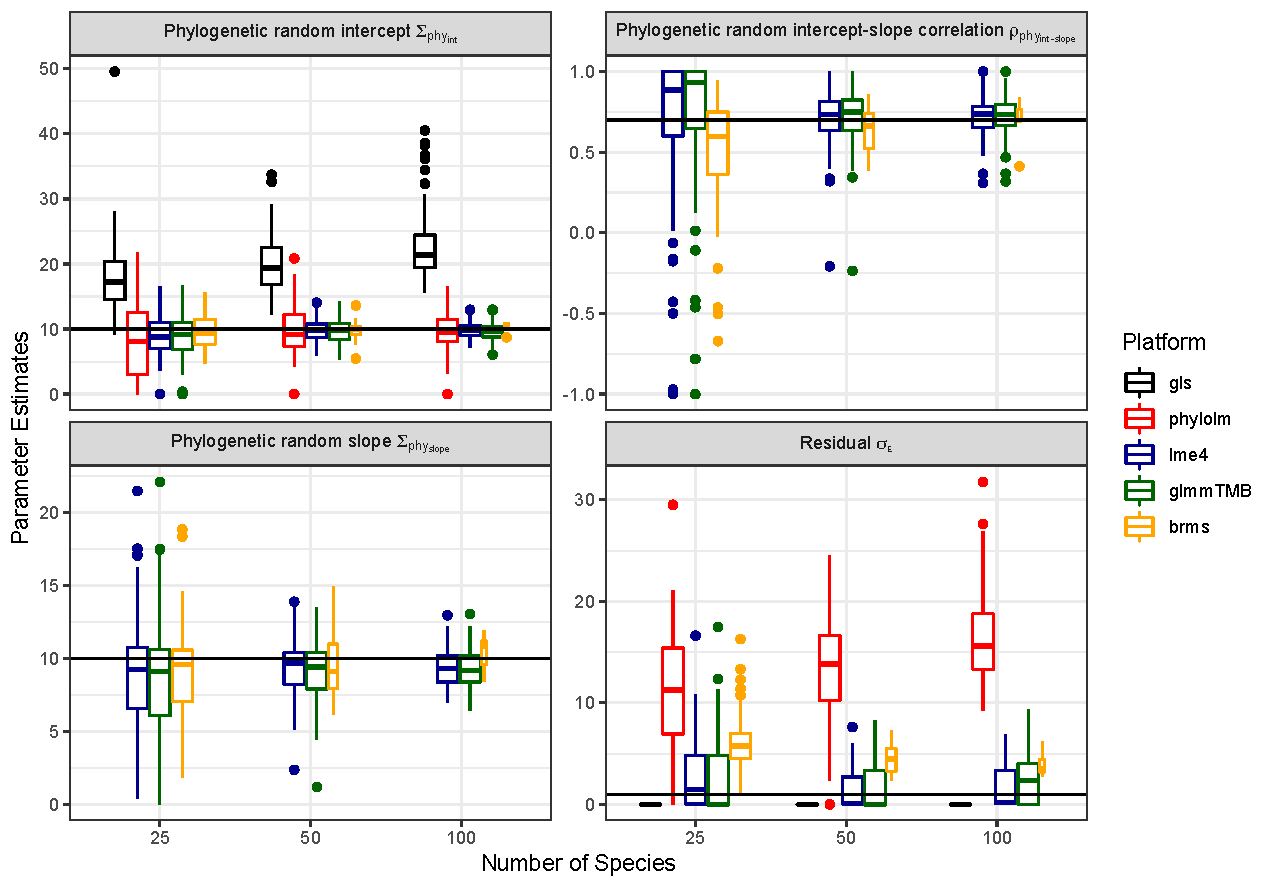
\includegraphics[scale=1]{./ssplot.pdf}
% \end{figure}
% \end{center}

\ml{add a paragraph about dune fits on real data}

\newpage

\section{Discussion}

We have fitted models including maximum capabilities to model varying levels of variation/phylogenetic signal to simulated data with our simple model with a single response and predictor variable.
Using models that can include/account for multiple levels of variation is necessary for robust fits, but models that include phylogenetic signal in the intercept level can work as well as the full model.
Under the Brownian motion evolution process assumption, modelling via independent errors is much more computationally efficient than imposing equivalent correlation structures.

\subsection{Process and residual (observation) variabilities and confoundings}

Process and observation errors are highly confounded in phylogenetic regression.
The effects of models that include both process and residual variations (i.e. pglmm, pglm) instead of the less realistic model that assumes variation due to evolution and zero observation (gls) was large. 
In particular, models that did not include residual variation tended to over-estimate the amount of variabilities in the evolution process. 
Thus, any model that can account for at least two sources of variation (one for the residual variance, and at least one for the process variation) will be sufficient to a first approximation (i.e. Pagel's lambda, Blomberg's K). 

\subsection{Random Slopes}

In classic GLMM (without phylogenetic relationships), random slopes models are not always appropriate, but they are relevant over a wider range of scenarios than people are currently thinking about \cite{schielzeth2013nested, cleasby2015quantifying}.
When analyzing evolutionary process among species between species traits and environmental variables, it is entirely plausible that the relationship across different traits and predictor variables are varying in a phylogenetically correlated way.
Although the effects of including phylogenetically correlated random slopes are relatively low compared to process and residual variation in the intercept, it is still useful and informative than ignoring it from the model.
It may be easier to simplify the phylogenetic relationships (at the random slopes level) and think about the random-slopes model in a strictly hierarchical setting (i.e., estimating different slopes for each family, or taxon \cite{ord2010adaptation}) - the PGLMM collapses to a standard random-slopes model. \ml{which would only be identifiable if ...}
However, in the PGLMM context, as long as there's variation in the predictor among tips, there will be variation among taxa at some level, so random-slopes models will (almost always) be *theoretically* identifiable.

\subsection{Extension and alternatives}

Our analysis covers the classical phylogenetic comparative methods (i.e. phylogenetic least squares, linear and mixed models).
Even within the scope there is additional room for exploration we neglected, such as exploring phylogenetic multivariate response models, non-BM evolution processes (such as Ornstein-Uhlenbeck (OU) process which accounts for both selection and drift processes \cite{butler2004phylogenetic}), Bayesian approaches \cite{hadfield2010general}.
More broadly, the simple independence error approach we developed here offers a more efficient and mathematical equivalent way to do Brownian motion evolution process phylogenetic comparative analysis. 
This approach can in principle be combined flexibly with the state of the art phylogenetic mixed models using platforms that supports independent latent variables such as MCMCglmm \cite{hadfield2010mcmc}; a widely used Bayesian approach to PGLMM.
However, in principle just like GLMM and most statistically models, users should be aware the amount of data they have and the complexity of the model they want to fit.
\ml{This note should go somewhere here: how much data do we need in order to practically estimate the random slopes? Are we making a mistake (cf Schielzeth) by ignoring random slopes? What should we do when we don't have enough data? (cf. Barr et al 2013 "keep it maximal"; Bates, Vashisth, etc etc who don't like that, possibility of Bayesian approaches, etc etc etc)}
More importantly, this implementation in lme4 allows users to fit phylogenetic mixed models to the fullest ( that other frequentest platforms lack of (i.e. large data, unbalance species observations, complex random effects) and explore new ideas.


\section{Conclusion}

We have presented a simple approach to fit phylogenetic mixed models that is both more efficient and statistically equivalent approach and comparison of classical PCM to simulated data. 
First, this new approach is magnitudes faster compared to existing phylogenetic mixed models without losing robustness/accuracy and can easily combined with any statistically mixed model framework. 
Last and most importantly, it is more flexible in fitting large phylogenies, large volume of data, unbalanced data sets, and complex random effects such as slope correlations.



\newpage

\section{Supplements -- translation}

$1 \mid Sp_{phylo}$, $0 + X_{E} \mid Sp_{phylo}$ and $X_{E} \mid Sp_{phylo}$ means phylogenetically related have similar response,   

\begin{tabularx}{\textwidth}{|l|X|X|}
\hline
Formula & Statistics & Biology \\
\hline
$1 \mid Sp$ &
random species intercept; variation within species in mean response across all factors &
variation of how species respond \\
\hline

$0 + X_{E} \mid Sp$ &
random slope of environment factor within species; variation in coefficient within species for the environmental factor &
variation of how species respond to the same environmental factor \\
\hline

$1 + X_{E} \mid Sp$ &
random slope of environmental factor within species with correlated intercept; variation in coefficient within species for the environmental factor with correlated mean response across all other factors &
variation of how species respond in the same environmental factors and the correlation of the variation of how they respond in general \\
\hline

$1 \mid Site:Sp $ &
random variation in intercept among species within sites &
variation of how species respond within sites \\
\hline

$1 | Sp_{Phylo} $ &
variation among species in mean response across all factors demonstrate phylogenetic signal &
phylogenetically related species respond similarly \\
\hline

$0 + X_{E} \mid Sp_{Phylo}$ &
variation among species for environmental factors demonstrate phylogenetic signal &
phylogenetically related species respond similar (share common response) to the same environmental factor \\
\hline
\end{tabularx}
            
                                                                        
